\section{Representations and fitted forecasting rules}
\label{sec:nf-methods}

A history $x\in\mathbb R^d$ contains the observations available at a forecast
origin; its response $y\in\mathbb R^H$ contains the next $H$ observations.
For the univariate tasks below, the input dimension $d$ equals the history length $L$.
We fit direct multioutput regressors to historical pairs
$\{(x_i,y_i)\}_{i=1}^n$.  The construction below specifies which part of the
regressor uses KAHM geometry.  It does not assume that overlapping forecasting
windows are independent.  All input transformations, reference sets, and
decoder bases are fitted on the training portion of each fit.

\subsection{Shared reference geometry}
\label{sec:nf-reference-geometry}

Write $z(x)=D^{-1}(x-\bar x)$, where $\bar x$ and the diagonal scales $D$ are
training means and population standard deviations.  A standard deviation at
most $10^{-12}$ is replaced by one.  Thus this transformation retains every
raw coordinate, including coordinates constant in the observed training set.
Three independently seeded $k$-means partitions, with $k\in\{2,4,8\}$, use
the same seeded subset of at most 512 training histories.  Each partition has
five initializations and at most 150 iterations.  Each cluster supplies at
most 24 references sampled without replacement; all its rows are used if
there are fewer.  For a common seed and training set, the alternative gates
use identical partition and reference-selection rules.  They are nevertheless
fitted as separate computational pipelines.

Index the 14 local models by $c$, with the partition blocks denoted
$\mathcal C_b$.  Let
$Q_c=[q_{c1},\ldots,q_{cm_c}]\in\mathbb R^{d\times m_c}$ contain the
training-standardized references, stored after the inherited float32
conversion, and let $\mu_c=m_c^{-1}Q_c\mathbf 1$.
The orthonormal columns of $P_c\in\mathbb R^{d\times r_c}$ are leading
eigenvectors of the centered reference covariance.  The requested rank is
$\min(2,d-1,m_c-1)$; only eigenvalues above double-precision machine epsilon
are retained.  The inherited implementation further reduces a rank greater
than one if the smallest projected coordinate range is below $10^{-3}$.
A reference set with no usable direction has $r_c=0$ and uses its center as
its reconstruction.  Other numerical failures remain recorded failures.

The affine reconstruction and centered local coordinates are
\begin{equation}
 a_c(z)=\mu_c+P_cP_c^\top(z-\mu_c),
 \qquad u_c(z)=P_c^\top(z-\mu_c).
 \label{eq:nf-affine}
\end{equation}
The affine and locality controls compute these quantities without fitting or
querying any KAHM kernel.

\subsection{Reconstruction scores and local gates}
\label{sec:nf-gates}

\paragraph{KAHM reconstruction.}
Kernel Affine Hull Machines construct nonlinear reconstructions from local
kernel weights \citep{Kumar2024KAHM}.  We retain the pinned implementation's
local autoencoder, rather than asserting equivalence to an independently
optimized end-to-end KAHM learner.  For $r_c>0$, let $\Sigma_c$ be the sample
covariance of the columns of $P_c^\top Q_c$.  Its Gaussian kernel is
\begin{equation}
 k_c(z,q)=\exp\!\left\{-\frac{
  (P_c^\top(z-q))^\top\Sigma_c^{-1}P_c^\top(z-q)}{2r_c}\right\},
 \qquad (K_c)_{ij}=k_c(q_{ci},q_{cj}).
 \label{eq:nf-kahm-kernel}
\end{equation}
To specify the inherited local regularizer exactly, put
$\nu_c=\|Q_c\|_F^2/(dm_c)$ and initialize $\lambda_0=5\nu_c/2$.  Its iteration is
\begin{equation}
 B_t=(K_c+\lambda_t I)^{-1},\qquad
 \lambda_{t+1}=2\nu_c+
 \frac{\|Q_c-Q_c(K_cB_t)^\top\|_F^2}{dm_c}.
 \label{eq:nf-local-regularizer}
\end{equation}
It stops after an update of size at most $10^{-3}$ or 100 updates, and
retains the last computed $B_t$ as $B_c$.  In particular, it does not perform
an extra inverse at the newly updated $\lambda_{t+1}$.
For $k_c(z)=(k_c(z,q_{cj}))_{j=1}^{m_c}$, define
\begin{equation}
 v_c(z)=B_c^\top k_c(z),\qquad
 \widehat z_c(z)=\frac{Q_cv_c(z)}{\mathbf 1^\top v_c(z)}.
 \label{eq:nf-reconstruction}
\end{equation}
The weights may be signed.  The reconstruction is therefore not generally a
convex average.  The inherited exact-zero-denominator convention replaces
the denominator by one; that convention is an implementation choice, not
a definition of a continuous extension at a singularity.

\paragraph{Stable Gaussian evaluation.}
For queries we compute the analytic log kernel
$\ell_{cj}(z)=-\|S_cP_c^\top(z-q_{cj})\|^2/(2r_c)$, where $S_c$ is the
stored symmetric square root of the inverse covariance, and use
$\widetilde k_{cj}(z)=\exp\{\ell_{cj}(z)-\max_j\ell_{cj}(z)\}$ in
Equation~\eqref{eq:nf-reconstruction}.
In exact arithmetic, $S_c^\top S_c=\Sigma_c^{-1}$, and multiplying every
kernel entry for one query by the same positive constant cancels from the
normalized reconstruction whenever its denominator is nonzero.
This calculation avoids underflow caused solely by a large common negative
log-kernel offset.  It does not prevent signed cancellation, guarantee a
well-conditioned denominator, or guarantee equivalence at an exact zero.
The implementation retains the zero-denominator convention, records numerical
diagnostics, and rejects nonfinite outputs.  The historical mode instead
exponentiates the unshifted logs through the inherited query routine; it is
retained for equivalence checks, while this study uses the shifted evaluation.

\paragraph{Matched folding gates.}
Given either the KAHM reconstruction $\widehat z_c$ or the affine
reconstruction $a_c$, denote it by $r_c^{\mathrm{rec}}(z)$.  Define
\begin{align}
 \rho_c(z)&=1-\exp\{-\|z-r_c^{\mathrm{rec}}(z)\|\},\qquad
 \theta_c(z)=\frac1\pi\arccos\!\left(
 \operatorname{clip}_{[-1,1]}
 \frac{z^\top r_c^{\mathrm{rec}}(z)}{\|z\|\,\|r_c^{\mathrm{rec}}(z)\|}\right),
 \notag\\
 s_c(z)&=\sqrt{\{\rho_c(z)^2+\theta_c(z)^2\}/2},\qquad
 \phi_c(z)=\frac{[1-\operatorname{clip}_{[0,1]}s_c(z)+\tau]^\omega}
 {\sum_{j\in\mathcal C_b}[1-\operatorname{clip}_{[0,1]}s_j(z)+\tau]^\omega},
 \quad c\in\mathcal C_b.
 \label{eq:nf-folding-gates}
\end{align}
When either norm in the cosine denominator is zero, its cosine is set to
zero, so that $\theta_c=1/2$.  The fixed values are $\omega=16$ and
$\tau=10^{-6}$; normalization is evaluated with log-sum-exp.  The comparison
between these two gates changes the reconstruction while retaining the
score, reference geometry, and local-coordinate construction.

\paragraph{Locality control.}
The third gate uses the historical native-affine score formula, applied to
the same references.  With $\epsilon=10^{-6}$, set
\begin{align}
 t_c&=\max\!\left\{m_c^{-1}\sum_j\|q_{cj}-\mu_c\|^2,\epsilon\right\},\notag\\
 e_c&=\max\!\left\{m_c^{-1}\sum_j\|q_{cj}-a_c(q_{cj})\|^2,
                    0.05t_c,\epsilon\right\},\notag\\
 b_c(z)&=\frac{\|z-a_c(z)\|^2}{e_c}
          +0.1\frac{\|z-\mu_c\|^2}{t_c},\notag\\
 \phi_c(z)&=\frac{\exp[-b_c(z)]}
                    {\sum_{j\in\mathcal C_b}\exp[-b_j(z)]}.
 \label{eq:nf-locality-gates}
\end{align}
This distinguishes proximity to the local center from projection residual.
Here ``native'' identifies a score formula; it does not identify a separately
tuned native learning algorithm.  It supplies a non-KAHM locality alternative
to the matched folding-score comparison.

\subsection{Local codes and finite forecasting heads}
\label{sec:nf-local-features}

For each gate family $g$, concatenate all gates and gated local coordinates:
\begin{equation}
 T_g(x)=\bigl((\phi_c(z(x)))_c,
                  (\phi_c(z(x))u_c(z(x)))_c\bigr),\qquad
 T_{\mathrm{raw}+g}(x)=(z(x),T_g(x)).
 \label{eq:nf-local-code}
\end{equation}
The stored local width is $14+\sum_c r_c\leq42$; the actual width is recorded.
The raw augmentation prepends all $d$ history coordinates, with no truncation
when $d>28$.  The combination of local association and local position is
related to coordinate and tangent coding \citep{Yu2009LCC,Yu2010LTC};
our gates and decoder are the explicit constructions above.
The stack of $P_c^\top$ has rank at most 28.  A deficient stack alone does
not prove information loss in $T_g$, because the gates also depend on the
query.  Raw augmentation gives the simpler unconditional reconstruction
property stated below, without a rank assumption.

\paragraph{Nystr\"om plus linear basis.}
\label{sec:nf-head}
Let $v(x)$ denote $z(x)$, $T_g(x)$, or $T_{\mathrm{raw}+g}(x)$, and let
$q(x)$ be its coordinatewise training standardization.  Select $M$ training
rows without replacement as landmarks $a_1,\ldots,a_M$ in $q$-space.
The requested $M$ is 32 or 64, capped by the training size.
Set $\sigma^2$ to the median positive squared inter-landmark distance and
define
\begin{equation}
 k_\sigma(q,a)=\exp\{-\|q-a\|^2/(2\sigma^2)\},\qquad
 b(x)=\left(q(x),\;
       \operatorname{diag}(\eta_J^{-1/2})U_J^\top
                  (k_\sigma(q(x),a_j))_{j=1}^M\right).
 \label{eq:nf-nystrom}
\end{equation}
Here $U\operatorname{diag}(\eta)U^\top$ diagonalizes the landmark Gram
matrix, and $J$ retains eigenvalues exceeding
$\max(10^{-10}\eta_{\max},10^{-12})$ \citep{Williams2001Nystrom}.
Distances at most $10^{-14}$ are excluded from the bandwidth median;
if none remain the squared bandwidth is one, and in all cases it is floored
at $10^{-12}$.  The bandwidth multiplier is fixed to one.
Finally, standardize $b$ on training rows to obtain $f(x)$ and the design
$F_{i,:}=f(x_i)^\top$.  Both head standardizations replace scales below
$10^{-8}$ by one.  Raw ridge omits the Nystr\"om block and uses the same
centering and scaling convention.

For each horizon $h$, the fitted decoder solves
\begin{equation}
 \min_{\beta_h,a_h}\ \frac1n\sum_{i=1}^n
       [y_{ih}-a_h-f(x_i)^\top\beta_h]^2+\alpha\|\beta_h\|^2.
 \label{eq:nf-ridge-objective}
\end{equation}
Thus the normal equations use $F^\top F/n+\alpha I$, and the intercept is
unpenalized.  Internally, targets are standardized using training statistics
and transformed back after prediction.  For fixed $\alpha$, linearity makes
this exactly equivalent in real arithmetic to
Equation~\eqref{eq:nf-ridge-objective} in the original target units.
This is a Euclidean ridge penalty on a standardized finite basis, rather
than the canonical Gaussian RKHS norm.  Adding local features also changes
the Gaussian distances and the resulting Nystr\"om basis; the raw and
augmented nonlinear decoder classes need not be nested.

One common $\alpha$ from the ordered grid $(0.01,1,100)$ is selected by validation MSE averaged
over origins and horizons in original target units, with the first grid
entry winning ties.  Within a method, geometry, training and validation
features, basis construction, and the Gram eigensystem are computed once;
all three alphas reuse those quantities.  Different method variants share
no fitted bank or free preprocessing.  The selected configuration is then
fitted anew on the admissible pretest training data.  Search designs and
eigensystems are not retained in the serialized final model.  This gives
an explicit efficient search whose full computation can be measured.

\subsection{Information and finite-decoder risk}
\label{sec:nf-information}

The following elementary facts delimit the interpretation of the experiments.
They are established information-preservation and linear-smoother algebra,
not new KAHM approximation theorems or performance guarantees.

\begin{proposition}[Information preserved by raw augmentation]
\label{prop:nf-raw-preservation}
Condition on a fitted state $\Theta$ containing $\bar x$, positive diagonal
$D$, and a measurable, finite-valued feature map $T_g$ on the support of $X$.
Then $T_{\mathrm{raw}+g}(X)$ and $X$ generate the same information conditional
on $\Theta$.  For a square-integrable response $Y$, their conditional
expectations and optimal squared-loss Bayes risks coincide, conditional on
$\Theta$.  This statement requires neither positive gates nor a full-rank
stack of local bases.
\end{proposition}
\begin{proof}
The augmented code is a measurable function of $(X,\Theta)$, and its first
$d$ coordinates recover $X=\bar x+Dz(X)$.  Consequently
$\sigma(T_{\mathrm{raw}+g}(X),\Theta)=\sigma(X,\Theta)$.
Conditional expectation onto these equal sigma-fields, and hence the
minimum squared prediction error, is identical.
\end{proof}

This is an exact-arithmetic statement about the representation, not a
conditioning guarantee or a claim that a particular fitted decoder uses
every retained coordinate.  Empirical gains from raw augmentation must
therefore be explained through finite fitting, representation-dependent
regularization, or numerical behavior, rather than increased Bayes
information relative to the same raw input.

\begin{proposition}[Fixed-feature, fixed-alpha risk identity]
\label{prop:nf-linear-risk}
Consider one response coordinate, a fixed $\alpha>0$, and the centered
training design $F$ above.  Let $\mathcal G$ contain the training and query
inputs and the randomness used to fit their unsupervised feature map, so
$F$ and $f(x_*)$ are $\mathcal G$-measurable.  Put
\begin{equation}
 w_* = \frac{\mathbf 1}{n}
       +F(F^\top F+n\alpha I)^{-1}f(x_*).
 \label{eq:nf-smoother}
\end{equation}
Let the training response vector be $Y$, the future response be $Y_*$, and
assume their conditional second moments are finite.  Define
$\mu=\mathbb E[Y\mid\mathcal G]$,
$\mu_*=\mathbb E[Y_*\mid\mathcal G]$,
$\Sigma=\operatorname{Cov}(Y\mid\mathcal G)$,
$c=\operatorname{Cov}(Y,Y_*\mid\mathcal G)$, and
$v_*=\operatorname{Var}(Y_*\mid\mathcal G)$.  The fitted prediction is
$\widehat Y_*=w_*^\top Y$, and
\begin{equation}
 \mathbb E[(\widehat Y_*-Y_*)^2\mid\mathcal G]
   =(w_*^\top\mu-\mu_*)^2+w_*^\top\Sigma w_*+v_*-2w_*^\top c.
 \label{eq:nf-dependent-risk}
\end{equation}
\end{proposition}
\begin{proof}
Because $F^\top\mathbf 1=0$, the unpenalized intercept is $\bar Y$ and
$\widehat\beta=(F^\top F+n\alpha I)^{-1}F^\top Y$.
Substituting into $\bar Y+f(x_*)^\top\widehat\beta$ gives
Equation~\eqref{eq:nf-smoother}; the inverse target standardization cancels
as described above.  Conditional on $\mathcal G$, expand the second moment
of $w_*^\top Y-Y_*$ as its squared mean plus its variance.  The covariance
cross term is $-2w_*^\top c$, giving the identity.
\end{proof}

The identity holds without independent training responses or an independent
future response.  Overlapping windows and serial dependence can affect both
$\Sigma$ and $c$; neither may be discarded without additional assumptions.
Averaging the identity over horizons gives the corresponding average risk.
Changing geometry changes $w_*$ and can change all its bias and covariance
terms, without a universal ordering between representations.  The identity
does not automatically describe the full validation-selected procedure:
after alpha selection, the smoother depends on observed validation responses.
No generalization or selection guarantee is inferred from it.

\section{Natural-data protocol}
\label{sec:nf-protocol}

Source allocation, task roster, model grids, and analysis are fixed before
comparative outcomes.  The evaluation compares matched representations, accuracy and computational
cost, and prospective model selection on reserved source families. The
reproduction materials include specifications, input checksums, and source
checkpoints. The study was not externally preregistered.

\subsection{Sources and chronological tasks}
\label{sec:nf-data}

Table~\ref{tab:nf-sources} gives eight versioned Monash snapshots
\citep{Godahewa2021Monash}, chosen by provenance, application diversity, length,
and size.  Related series, channels, and aggregations share a source family
and cannot cross the boundary between development and confirmation.  Models are local to
each series, including differently dated Tourism series.  The supplement
retains the records' CC BY 4.0 licenses, versions, attribution, original-source
references, and archive hashes.

\begin{table}[t]
\caption{Fixed source allocation and forecast regimes.  ``Selected/all'' counts
series, not independent source families.  Each selected series uses both regimes
for its frequency.  $L$ is history length, $H$ forecast horizon, and $s$ the
declared seasonal period.}
\label{tab:nf-sources}
\centering\small
\setlength{\tabcolsep}{4pt}
\begin{tabular}{@{}lp{0.48\linewidth}cr@{}}
\toprule
Phase & Source snapshot & Frequency & Selected/all \\
\midrule
Development & Electricity \citep{DatasetElectricityWeekly} & weekly & 4/321 \\
 & NN5, with missing values \citep{DatasetNN5Daily} & daily & 4/111 \\
 & Tourism \citep{DatasetTourismMonthly} & monthly & 4/366 \\
 & FRED-MD \citep{DatasetFREDMD} & monthly & 4/107 \\
\midrule
Confirmation & Traffic \citep{DatasetTrafficWeekly} & weekly & 4/862 \\
 & Hospital \citep{DatasetHospitalMonthly} & monthly & 4/767 \\
 & Saugeen River flow \citep{DatasetSaugeenDaily} & daily & 1/1 \\
 & US births \citep{DatasetUSBirthsDaily} & daily & 1/1 \\
\bottomrule
\end{tabular}
\par\medskip
\begin{tabular}{@{}lccc@{}}
\toprule
Frequency & Short $(L,H)$ & Long $(L,H)$ & $s$ \\
\midrule
Monthly & $(12,3)$ & $(24,6)$ & 12 \\
Weekly & $(13,4)$ & $(26,8)$ & 52 \\
Daily & $(28,7)$ & $(56,14)$ & 7 \\
\bottomrule
\end{tabular}
\end{table}

Training-prefix eligibility requires at least 16 finite windows in each regime
and a positive training error scale.  A fixed salted hash of source and series
ID orders eligible series; we retain the first four, or all if fewer exist,
across regimes and capacities.  No later loss or availability criterion selects
replacements.  The 26 series give 52 base tasks; two capacities and seeds 17
and 43 give 208 runs: 128 development and 80 confirmation, with four source
families per phase.

For a length-$n$ series indexed from zero, let
$a=\lfloor3n/5\rfloor$ and $b=\lfloor4n/5\rfloor$.  Training, validation, and
test intervals are $[0,a)$, $[a,b)$, and $[b,n)$.  An origin $t$ is the last
observed index, with
\begin{equation}
 x_t=(y_{t-L+1},\ldots,y_t)^\top,\qquad
 y_t^+=(y_{t+1},\ldots,y_{t+H})^\top.
 \label{eq:nf-forecast-window}
\end{equation}
The complete target interval must lie within its split; contexts may include
earlier observed values.  Stateful controls receive $t+1$, their first-future
index.  We retain raw snapshot values, including NN5 missing markers, and
discard windows with an unavailable context or target without interpolation.
Evenly spaced indices among available origins give at most 64 validation and
64 test windows, and the training cap in Table~\ref{tab:nf-capacity}.  Every
method receives the same evaluation origins.

Before outcomes, length checks reduced the proposed monthly $(48,6)$ and
weekly $(52,8)$ regimes, which yield zero Hospital and three Traffic training
windows.  The adopted long regimes yield 21 and 29, respectively.  Context
and horizon are paired, so their separate effects are not identified.
NN5 T88 at $(56,14)$ retains only seven test origins out of 146 candidates.
All task availability counts are recorded.

All candidate preprocessing is fitted on training data, and validation MSE
selects hyperparameters.  The selected pipeline is then fitted anew on all
eligible windows with targets preceding $b$, subject to its training cap.
This refit includes windows crossing the former training/validation
boundary because all their targets precede the test segment.  Parameters are fixed thereafter; earlier realized observations may
enter later contexts or state updates.  Test outcomes never retune parameters.

\subsection{Comparators, capacity, and loss}
\label{sec:nf-comparators}

The twelve methods comprise raw ridge and raw RBF heads; affine-, locality-,
and KAHM-gated local RBF pipelines; each local pipeline augmented by the full
raw history; and seasonal naive, Holt, histogram gradient boosting, and a
one-hidden-layer MLP.  Section~\ref{sec:nf-methods} defines the feature maps and
finite RBF head.  The primary matched pair is raw RBF ($R$) versus raw-history
plus KAHM RBF ($K$).  The raw-history controls retain the inputs independently
of local-basis rank (Proposition~\ref{prop:nf-raw-preservation}).  The evaluation reports every method in this twelve-method portfolio.

The geometric bank uses cluster counts $(2,4,8)$, requested rank two, at most
24 references per local model, a 512-row fitting cap, $\omega=16$, and
$\tau=10^{-6}$.  Reduced effective ranks and numerical fallbacks are recorded.
Each alternative constructs its own representation; affine/locality controls
do not fit a KAHM kernel.  Within a method, the fixed representation and head
statistics are reused across ridge penalties $\{0.01,1,100\}$; the bandwidth
multiplier is one.  Boosting/MLP regularization is chosen from $\{0.01,1\}$,
Holt selects damped or undamped trend, and seasonal naive has no tuned parameter.
These modest declared grids do not imply optimal tuning of every comparator.

\begin{table}[t]
\caption{Capacity caps.  These are limits on examples and model size, not equal
realized time budgets.  A shorter source uses its available examples.}
\label{tab:nf-capacity}
\centering\small
\setlength{\tabcolsep}{5pt}
\begin{tabular}{@{}lrrrr@{}}
\toprule
Setting & Training windows & RBF landmarks & Tree leaves/iterations & MLP width/iterations \\
\midrule
Small & 512 & 32 & 15/100 & 32/200 \\
Medium & 1,024 & 64 & 31/150 & 64/300 \\
\bottomrule
\end{tabular}
\end{table}

Seasonal naive can use its declared lag from the observed past even when it
exceeds $L$, using the last finite value for an unavailable lag and period one
before a full seasonal lag exists.  Holt fits a capped historical segment,
forward-fills only within that segment, and assimilates observations strictly
before each forecast; an absent online observation causes a state prediction
without measurement update.  Boosting and MLP fit direct multi-output forecasts
without a random internal validation split.

For a nonempty set $\mathcal O$ of evaluated forecast origins, the
scaled task loss is
\begin{equation}
 \ell=\frac{1}{|\mathcal O|Hq}
       \sum_{t\in\mathcal O}\sum_{h=1}^{H}
       (\widehat y_{t+h}-y_{t+h})^2,
 \label{eq:nf-scaled-loss}
\end{equation}
Here $q$ is fitted on the uncapped initial training prefix. For seasonal
period $s$, let $\mathcal P_s$ contain indices for which both $y_i$ and
$y_{i-s}$ are finite observations in that prefix. The seasonal scale is
$q_s=|\mathcal P_s|^{-1}\sum_{i\in\mathcal P_s}(y_i-y_{i-s})^2$
when at least two such pairs exist. We use $q=q_s$ if this value is
positive and finite; otherwise we apply the same rule with $s=1$. A
series with neither valid scale is ineligible.  This denominator remains fixed during refitting.  Raw MSE,
$q$, predictions, and origin losses are saved and independently checked.

For each source family, we average seeds and capacities within each
history--horizon regime, then regimes within each series, and finally
series within the family. The overall mean weights source families equally.  These nested observations are not
independent source replications.  We report family outcomes, dispersion, and
leave-one-family-out sensitivity, without broad-population confidence intervals
or window-level significance claims.

\subsection{Measured pipeline and selector costs}
\label{sec:nf-costs}

Methods execute sequentially in fresh child processes with one BLAS thread
and deterministically shuffled order, limited to 120 seconds per method and
1,800 per task.  Wall and process CPU time are separate.  Each warm-library
scientific pipeline includes
data/checksum preparation, array loading, configuration fitting and validation,
selection bookkeeping, selected refitting, forecasting, and model serialization.
Source preparation is equally allocated across its tasks and charged consistently
to alternatives.  Shared imports are initialized before measurement;
initialization, process launch/IPC, and launch-to-result duration are recorded
separately rather than allocated arbitrarily to policies.

Let $S_m$ be the set of computational steps for searching method $m$
and $F_m$ the steps for its final refit, forecasts, and serialization.
Let $\mathcal D_{\rm data}$ contain shared data preparation steps,
$c_v$ be the measured cost of step $v$, and $c_{\rm decision}$ the
selection bookkeeping cost. A validation selector over candidate set
$\mathcal A$ chooses method $m^*$ and incurs
\begin{equation}
 \mathcal D_{\rm val}=\mathcal D_{\rm data}
      \cup\bigcup_{m\in\mathcal A}S_m\cup F_{m^*},\qquad
 C=\sum_{v\in\mathcal D_{\rm val}}c_v+c_{\rm decision}.
 \label{eq:nf-selector-cost}
\end{equation}
Set unions count shared dependencies once.  A learned selector instead pays
for its required metadata/geometry/probe nodes plus $S_{m^*}\cup F_{m^*}$,
even when it rejects KAHM.  Geometry-only acquisition is conservatively billed
through its measured fitted-probe component.  Thus policy costs are
counterfactual sums of measured required computations, not the cost of running
every alternative in the benchmark.

Development-label acquisition also costs the $R,K$ searches, refits, and
forecasts, plus each variant's feature/probe nodes.  We report this investment
separately from regression fitting, online policy costs, and the full research
benchmark's elapsed time, without assuming a deployment count for amortization.
Summed standalone task costs are conservative where sharing across seeds or
capacities could reduce work.

We also record serialized model bytes and peak process resident set
size (RSS).  RSS includes the
interpreter, arrays present at worker initialization, and earlier process history; it is neither
incremental memory nor an additive exact policy-memory reconstruction.  No
GPU measurement is inferred from CPU timing.  Failed attempts remain visible
and retain the available timing records.  Method failures are included in the coverage accounting before losses
are aggregated over the specified task and method roster.

\subsection{Prospective benefit diagnostic}
\label{sec:nf-diagnostic}

The diagnostic predicts benefit before a task's test outcomes, while using
its training history and permitted validation information.  Its development
label is $\log[(\ell_R+\epsilon)/(\ell_K+\epsilon)]$, with
$\epsilon=10^{-12}$.  Development test errors may train this cross-task rule;
confirmation errors cannot train, standardize, tune, or select it.

We retain four weighted ridge rules: metadata $M$, $M$ plus geometry $G$,
$M$ plus a validation probe $P$, and $M+P+G$.  With $N_{\rm train}$ denoting the number of retained training windows,
the metadata features are $\log(1+N_{\rm train})$, $\log(1+H/L)$, and training-prefix lag-one
autocorrelation, computed from finite adjacent observation pairs and set
to zero if either variance is zero or fewer than three pairs are available.
Geometry adds normalized KAHM gate entropy and $\log(1+r)$. For
$n_p$ probe-training inputs $z_i\in\R^d$ and the three partition
blocks $\mathcal C_b$, these quantities are
\[
 E_{\rm gate}=-\frac{1}{3n_p}\sum_{b=1}^3\sum_{i=1}^{n_p}
 \frac{\sum_{c\in\mathcal C_b}\phi_c(z_i)\log\phi_c(z_i)}
 {\log|\mathcal C_b|},\qquad
 r=\frac{1}{3n_pd}\sum_{b=1}^3\sum_{i=1}^{n_p}
 \sum_{c\in\mathcal C_b}\phi_c(z_i)\|z_i-a_c(z_i)\|_2^2.
\]
The gates and affine reconstructions are defined in
Appendix~\ref{sec:nf-methods}. A singleton block would contribute
zero normalized entropy.  The probe fits the matched $R,K$ pair with at most 128 training
windows, 16 landmarks, a 128-row bank cap, and penalty one; its feature is
the log ratio of scaled validation losses with the same loss floor.

The diagnostic penalty is fixed at one, with an unpenalized intercept.
Source-balanced feature standardization and fitting occur inside each
development fold, holding out an entire source family.  All four variants are
then fitted on all development families and frozen before confirmation.
The primary incremental comparison is $M+P+G$ against $M+P$, testing whether
geometry adds value beyond metadata and a reduced-capacity validation probe.
Controls include always $R$, always $K$, direct probe selection, validation
selection within the matched pair, the six-method raw/practical portfolio,
the two-method KAHM portfolio, and the full twelve-method portfolio.

A positive predicted log benefit selects $K$; zero or negative estimates
select $R$.  A fixed 5\%
relative MSE change defines secondary practical benefit/harm, not a tuned
selection threshold.  All four variants are reported without choosing one from
confirmation performance.  A test-set oracle is only a hindsight regret
reference.  Utility requires improved held-out loss--cost behavior against
metadata and probe controls, not merely correlation with retrospective gains.

Before confirmation, a verification program checks development predictions
against their targets and reported errors. The archived checkpoint records
the code, dependencies, task roster, development records, and diagnostic
coefficients. Confirmation evaluates the complete specified roster.
This is a selected, small collection, not a random sample of forecasting
domains or a state-of-the-art survey.  Seasonal periods are conventions rather
than fitted optimal cycles.  In particular, FRED-MD is a fixed-vintage
snapshot: its metadata describe transformed series without a complete
per-series preprocessing audit \citep{DatasetFREDMD}.  Our train-only guarantees
apply to processing in this extension, not to unverified upstream decisions,
historical revisions, or release-time availability.  The conclusions must
remain conditional on these sources, contexts, grids, and resource settings.


\section{Additional natural-source results and diagnostics}\label{app:full-results}
The following tables retain all declared methods, selection policies, source
means, capacities, diagnostic variants, and recorded fitting warnings.
These are descriptive summaries under the same fixed source hierarchy.
They do not pool the natural-source results with the controlled-study
confidence families. Full precision, forecasts, targets, origins, selected
parameters, and cost components are retained in the anonymous supplement.
\begin{table}[t]
\centering\small\setlength{\tabcolsep}{4pt}
\caption{Standalone confirmation methods, equally weighted across 4 original source families using the frozen within-source hierarchy. Loss is training-scale-normalized MSE. Wall and CPU seconds cover complete warm-library scientific pipelines. RSS is the averaged maximum recorded process high-water mark, not incremental memory; model size is serialized bytes in KiB. No uncertainty intervals are inferred from dependent tasks.}\label{tab:method-summary}
\begin{tabular}{lrrrrr}
\toprule
Method & Scaled MSE & Wall (s) & CPU (s) & RSS (MiB) & Model (KiB) \\
\midrule
Raw ridge & 0.7798 & 0.188 & 0.1879 & 171.5 & 5.655 \\
Raw RBF & 0.8075 & 0.1688 & 0.1687 & 171.5 & 37.32 \\
Affine local & 0.9449 & 0.5002 & 0.4897 & 171.5 & 93.2 \\
Locality local & 0.8964 & 0.2898 & 0.2898 & 171.5 & 93.4 \\
KAHM local & 0.9354 & 0.3218 & 0.3214 & 171.5 & 164.6 \\
Raw + affine & 0.8458 & 0.3379 & 0.3265 & 171.5 & 107.8 \\
Raw + locality & 0.8462 & 0.2791 & 0.279 & 171.5 & 107.8 \\
Raw + KAHM & 0.8419 & 0.3874 & 0.3814 & 171.5 & 179.2 \\
Seasonal naive & 1.05 & 0.1614 & 0.1613 & 171.5 & 0.1382 \\
Holt & 2.373 & 0.3449 & 0.3446 & 171.5 & 0.4219 \\
Histogram boosting & 0.9555 & 8.91 & 8.901 & 171.5 & 2591 \\
MLP & 0.8785 & 1.463 & 1.462 & 171.5 & 71.62 \\
\bottomrule
\end{tabular}
\end{table}

\begin{table}[t]
\centering\small\setlength{\tabcolsep}{4pt}
\caption{Confirmation cost transparency for the primary matched pair, with equal source-family weighting. Total is the complete warm-library scientific pipeline. Cleanup is its measured selection-overhead component, including explicit garbage collection; the percentage is the ratio of aggregated component and total times. Launch separately reports the measured isolated-child launch-to-result interval. These are implementation-specific costs, not intrinsic kernel arithmetic or universal complexity ratios.}\label{tab:cleanup-costs}
\begin{tabular}{lrrrr}
\toprule
Method & Total (s) & Cleanup (s) & Cleanup (\%) & Launch (s) \\
\midrule
Raw RBF & 0.16879 & 0.13808 & 81.8 & 0.17748 \\
Raw + KAHM & 0.38741 & 0.18253 & 47.11 & 0.40097 \\
\bottomrule
\end{tabular}
\end{table}

\begin{table}[t]
\centering\small\setlength{\tabcolsep}{4pt}
\caption{Frozen-policy confirmation outcomes over 4 source families with the same hierarchical weighting. Gain is raw-RBF scaled MSE minus chosen loss. Harm is the weighted fraction with loss more than 5\% above raw RBF. The final column counts selection of the specific raw-plus-KAHM pair member, including in portfolios. Wall cost includes all required probes/searches and decision inference, then the chosen final refit, forecast and model serialization. Offline evidence acquisition and diagnostic fitting are separate.}\label{tab:policy-summary}
\begin{tabular}{lrrrrr}
\toprule
Policy & Scaled MSE & Wall (s) & Gain & Harm (\%) & Raw+K (\%) \\
\midrule
Always raw & 0.8075 & 0.1688 & 0 & 0 & 0 \\
Always raw + KAHM & 0.8419 & 0.3874 & -0.0344 & 25 & 100 \\
Validation: matched pair & 0.8097 & 0.4812 & -0.002159 & 5.47 & 32 \\
Validation: raw portfolio & 0.8639 & 8.338 & -0.05638 & 10.9 & 0 \\
Validation: KAHM family & 0.8406 & 0.6242 & -0.03306 & 26.6 & 73.4 \\
Validation: full portfolio & 0.8764 & 9.948 & -0.0689 & 14.8 & 14.1 \\
Cheap probe & 0.8143 & 0.3465 & -0.006771 & 9.38 & 50 \\
Metadata & 0.816 & 0.2976 & -0.008445 & 15.6 & 50 \\
Metadata + geometry & 0.816 & 0.3695 & -0.008445 & 15.6 & 50 \\
Metadata + probe & 0.8071 & 0.3309 & 0.0004363 & 3.12 & 31.2 \\
Metadata + probe + geometry & 0.8071 & 0.3309 & 0.0004363 & 3.12 & 31.2 \\
\bottomrule
\end{tabular}
\end{table}


\begin{figure}[t]
\centering
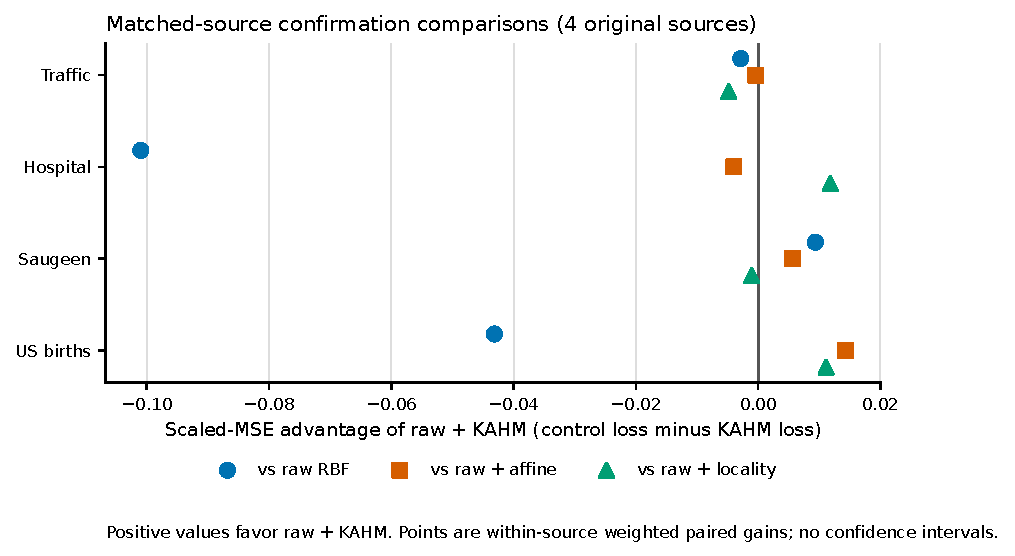
\includegraphics[width=\linewidth]{generated/natural/figures/source_gains.pdf}
\caption{Within-source confirmation comparisons. Positive differences favor
raw plus KAHM. Points compare the same hierarchically weighted source means;
no window-level uncertainty intervals are inferred. The small KAHM differences
against structural controls change sign across sources.}\label{fig:source-gains}
\end{figure}
\begin{figure}[t]
\centering
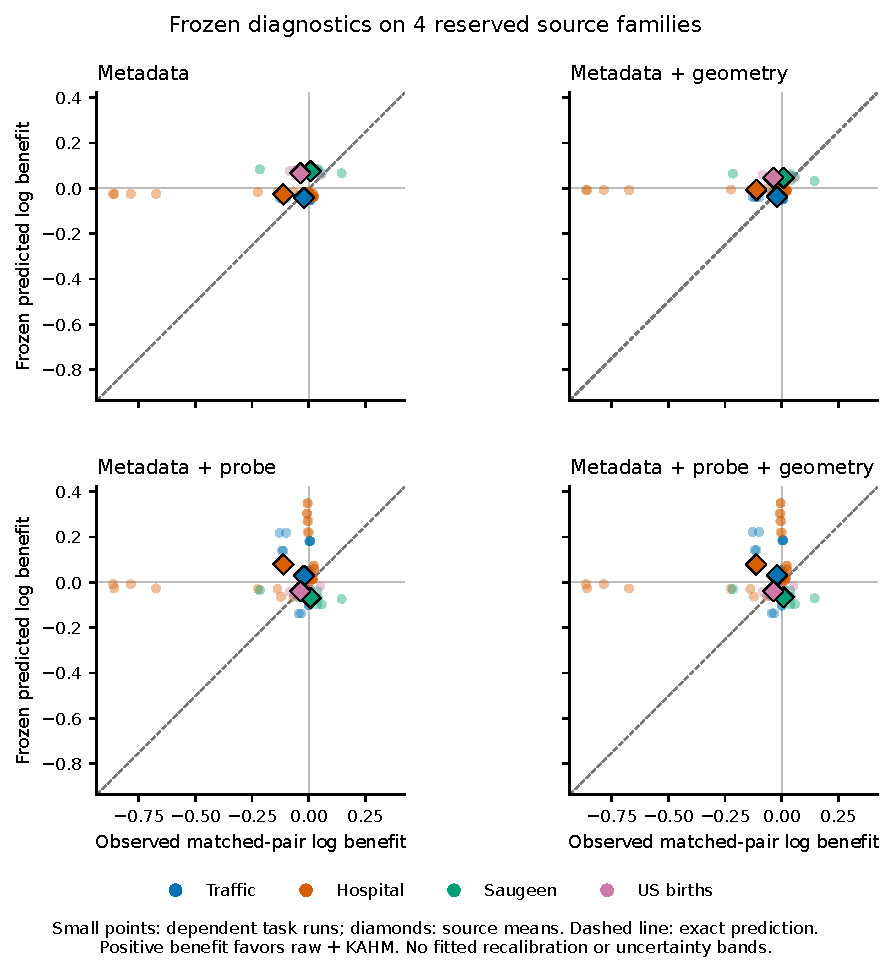
\includegraphics[width=0.92\linewidth]{generated/natural/figures/diagnostic_predictions.pdf}
\caption{Observed versus frozen predicted log benefit. Points within a source
are dependent task runs, and diamonds are source means. No recalibration is
fitted on confirmation. Similar decisions can coexist with different estimated
benefit magnitudes.}\label{fig:diagnostic-predictions}
\end{figure}
\FloatBarrier
{\small\setlength{\tabcolsep}{4pt}
\begin{longtable}{lrrrrr}
\caption{Development scaled MSE by original source family. The final column gives equal-source aggregation; source columns retain the declared within-source weights. Development diagnostics use leave-one-source-family-out fits; confirmation diagnostics use the frozen development fit. Always-policy rows duplicate their corresponding standalone methods deliberately.}\label{tab:source-development-loss}\\
\toprule
Method or policy & FRED-MD & NN5 & Tourism & Electricity & Equal-source \\
\midrule
\endfirsthead
\toprule
Method or policy & FRED-MD & NN5 & Tourism & Electricity & Equal-source \\
\midrule
\endhead
Raw ridge & 0.5601 & 0.8584 & 2.865 & 0.4243 & 1.177 \\
Raw RBF & 10.46 & 0.7552 & 3.476 & 0.4388 & 3.783 \\
Affine local & 2.548 & 0.8795 & 3.769 & 0.4535 & 1.912 \\
Locality local & 23.83 & 0.8148 & 3.778 & 0.4112 & 7.209 \\
KAHM local & 12.23 & 0.9163 & 3.636 & 0.4525 & 4.309 \\
Raw + affine & 1.409 & 0.7614 & 3.172 & 0.4481 & 1.448 \\
Raw + locality & 10.18 & 0.7474 & 3.046 & 0.4418 & 3.603 \\
Raw + KAHM & 4.254 & 0.7704 & 3.229 & 0.4539 & 2.177 \\
Seasonal naive & 2.269 & 1.089 & 2.982 & 0.5507 & 1.723 \\
Holt & 0.2409 & 1.358 & 8.228 & 0.6984 & 2.631 \\
Histogram boosting & 34.02 & 0.8032 & 4.786 & 0.4404 & 10.01 \\
MLP & 1.022 & 0.8475 & 2.77 & 0.4715 & 1.278 \\
Always raw & 10.46 & 0.7552 & 3.476 & 0.4388 & 3.783 \\
Always raw + KAHM & 4.254 & 0.7704 & 3.229 & 0.4539 & 2.177 \\
Validation: matched pair & 5.267 & 0.7335 & 3.229 & 0.4415 & 2.418 \\
Validation: raw portfolio & 0.2409 & 0.8021 & 3.014 & 0.4528 & 1.127 \\
Validation: KAHM family & 4.104 & 0.7792 & 3.223 & 0.4572 & 2.141 \\
Validation: full portfolio & 0.2409 & 0.8052 & 3.092 & 0.4675 & 1.152 \\
Cheap probe & 5.106 & 0.742 & 3.25 & 0.4217 & 2.38 \\
Metadata & 4.254 & 0.7704 & 3.229 & 0.4539 & 2.177 \\
Metadata + geometry & 4.254 & 0.7704 & 3.394 & 0.4539 & 2.218 \\
Metadata + probe & 4.157 & 0.759 & 3.338 & 0.4342 & 2.172 \\
Metadata + probe + geometry & 4.215 & 0.7704 & 3.338 & 0.4342 & 2.189 \\
\bottomrule
\end{longtable}
}

{\small\setlength{\tabcolsep}{4pt}
\begin{longtable}{lrrrrr}
\caption{Development warm-library wall seconds by original source family. The final column gives equal-source aggregation; source columns retain the declared within-source weights. Development diagnostics use leave-one-source-family-out fits; confirmation diagnostics use the frozen development fit. Always-policy rows duplicate their corresponding standalone methods deliberately.}\label{tab:source-development-cost}\\
\toprule
Method or policy & FRED-MD & NN5 & Tourism & Electricity & Equal-source \\
\midrule
\endfirsthead
\toprule
Method or policy & FRED-MD & NN5 & Tourism & Electricity & Equal-source \\
\midrule
\endhead
Raw ridge & 0.3731 & 0.1631 & 0.1888 & 0.1873 & 0.2281 \\
Raw RBF & 0.1929 & 0.1912 & 0.1834 & 0.1692 & 0.1842 \\
Affine local & 0.3285 & 0.2805 & 0.2983 & 0.2863 & 0.2984 \\
Locality local & 0.5431 & 0.29 & 0.2784 & 0.2649 & 0.3441 \\
KAHM local & 0.3705 & 0.3696 & 0.3735 & 0.3369 & 0.3626 \\
Raw + affine & 0.2923 & 0.2998 & 0.2979 & 0.288 & 0.2945 \\
Raw + locality & 0.3185 & 0.2967 & 0.2988 & 0.2533 & 0.2918 \\
Raw + KAHM & 0.4275 & 0.3807 & 0.3252 & 0.3024 & 0.3589 \\
Seasonal naive & 0.2125 & 0.177 & 0.1834 & 0.1878 & 0.1902 \\
Holt & 0.3224 & 0.42 & 0.3682 & 0.316 & 0.3567 \\
Histogram boosting & 3.086 & 4.954 & 1.729 & 1.819 & 2.897 \\
MLP & 1.278 & 0.9551 & 0.8521 & 0.5508 & 0.9089 \\
Always raw & 0.1929 & 0.1912 & 0.1834 & 0.1692 & 0.1842 \\
Always raw + KAHM & 0.4275 & 0.3807 & 0.3252 & 0.3024 & 0.3589 \\
Validation: matched pair & 0.5562 & 0.5313 & 0.4929 & 0.4301 & 0.5026 \\
Validation: raw portfolio & 4.066 & 5.306 & 2.641 & 2.719 & 3.683 \\
Validation: KAHM family & 0.692 & 0.6568 & 0.6115 & 0.5511 & 0.6278 \\
Validation: full portfolio & 5.861 & 6.513 & 4.138 & 4.075 & 5.147 \\
Cheap probe & 0.4739 & 0.4615 & 0.4004 & 0.3328 & 0.4172 \\
Metadata & 0.4284 & 0.3815 & 0.3258 & 0.3031 & 0.3597 \\
Metadata + geometry & 0.5195 & 0.465 & 0.3474 & 0.3744 & 0.4266 \\
Metadata + probe & 0.5029 & 0.474 & 0.2891 & 0.3411 & 0.4018 \\
Metadata + probe + geometry & 0.5284 & 0.4828 & 0.2891 & 0.341 & 0.4103 \\
\bottomrule
\end{longtable}
}

{\small\setlength{\tabcolsep}{4pt}
\begin{longtable}{lrrrrr}
\caption{Confirmation scaled MSE by original source family. The final column gives equal-source aggregation; source columns retain the declared within-source weights. Development diagnostics use leave-one-source-family-out fits; confirmation diagnostics use the frozen development fit. Always-policy rows duplicate their corresponding standalone methods deliberately.}\label{tab:source-confirmation-loss}\\
\toprule
Method or policy & Traffic & Hospital & Saugeen & US births & Equal-source \\
\midrule
\endfirsthead
\toprule
Method or policy & Traffic & Hospital & Saugeen & US births & Equal-source \\
\midrule
\endhead
Raw ridge & 0.5737 & 0.8461 & 0.522 & 1.177 & 0.7798 \\
Raw RBF & 0.5739 & 0.8228 & 0.6106 & 1.223 & 0.8075 \\
Affine local & 0.5796 & 0.928 & 0.6462 & 1.626 & 0.9449 \\
Locality local & 0.5719 & 0.7702 & 0.6504 & 1.593 & 0.8964 \\
KAHM local & 0.5775 & 0.9029 & 0.6652 & 1.596 & 0.9354 \\
Raw + affine & 0.5764 & 0.9198 & 0.6068 & 1.28 & 0.8458 \\
Raw + locality & 0.572 & 0.9356 & 0.6002 & 1.277 & 0.8462 \\
Raw + KAHM & 0.5768 & 0.9238 & 0.6012 & 1.266 & 0.8419 \\
Seasonal naive & 0.6484 & 0.7848 & 1.023 & 1.743 & 1.05 \\
Holt & 0.6842 & 1.003 & 0.6079 & 7.197 & 2.373 \\
Histogram boosting & 0.6524 & 1.025 & 0.5386 & 1.606 & 0.9555 \\
MLP & 0.6811 & 1.15 & 0.5365 & 1.147 & 0.8785 \\
Always raw & 0.5739 & 0.8228 & 0.6106 & 1.223 & 0.8075 \\
Always raw + KAHM & 0.5768 & 0.9238 & 0.6012 & 1.266 & 0.8419 \\
Validation: matched pair & 0.5738 & 0.8236 & 0.6042 & 1.237 & 0.8097 \\
Validation: raw portfolio & 0.6087 & 1.116 & 0.5639 & 1.167 & 0.8639 \\
Validation: KAHM family & 0.577 & 0.9182 & 0.6012 & 1.266 & 0.8406 \\
Validation: full portfolio & 0.6122 & 1.099 & 0.5695 & 1.225 & 0.8764 \\
Cheap probe & 0.5761 & 0.8211 & 0.6253 & 1.235 & 0.8143 \\
Metadata & 0.5739 & 0.8228 & 0.6012 & 1.266 & 0.816 \\
Metadata + geometry & 0.5739 & 0.8228 & 0.6012 & 1.266 & 0.816 \\
Metadata + probe & 0.5761 & 0.8189 & 0.6106 & 1.223 & 0.8071 \\
Metadata + probe + geometry & 0.5761 & 0.8189 & 0.6106 & 1.223 & 0.8071 \\
\bottomrule
\end{longtable}
}

{\small\setlength{\tabcolsep}{4pt}
\begin{longtable}{lrrrrr}
\caption{Confirmation warm-library wall seconds by original source family. The final column gives equal-source aggregation; source columns retain the declared within-source weights. Development diagnostics use leave-one-source-family-out fits; confirmation diagnostics use the frozen development fit. Always-policy rows duplicate their corresponding standalone methods deliberately.}\label{tab:source-confirmation-cost}\\
\toprule
Method or policy & Traffic & Hospital & Saugeen & US births & Equal-source \\
\midrule
\endfirsthead
\toprule
Method or policy & Traffic & Hospital & Saugeen & US births & Equal-source \\
\midrule
\endhead
Raw ridge & 0.1454 & 0.1959 & 0.1905 & 0.2204 & 0.188 \\
Raw RBF & 0.1644 & 0.1636 & 0.1693 & 0.1779 & 0.1688 \\
Affine local & 0.2424 & 0.2732 & 0.4038 & 1.082 & 0.5002 \\
Locality local & 0.2311 & 0.254 & 0.4021 & 0.2721 & 0.2898 \\
KAHM local & 0.2579 & 0.2764 & 0.3496 & 0.4035 & 0.3218 \\
Raw + affine & 0.3969 & 0.2809 & 0.354 & 0.3199 & 0.3379 \\
Raw + locality & 0.2223 & 0.2752 & 0.3166 & 0.3022 & 0.2791 \\
Raw + KAHM & 0.2674 & 0.4235 & 0.4676 & 0.3911 & 0.3874 \\
Seasonal naive & 0.1551 & 0.164 & 0.1874 & 0.1393 & 0.1614 \\
Holt & 0.2759 & 0.3535 & 0.4118 & 0.3386 & 0.3449 \\
Histogram boosting & 1.774 & 1.39 & 17.59 & 14.89 & 8.91 \\
MLP & 0.4046 & 0.392 & 2.264 & 2.79 & 1.463 \\
Always raw & 0.1644 & 0.1636 & 0.1693 & 0.1779 & 0.1688 \\
Always raw + KAHM & 0.2674 & 0.4235 & 0.4676 & 0.3911 & 0.3874 \\
Validation: matched pair & 0.3909 & 0.5408 & 0.5273 & 0.4656 & 0.4812 \\
Validation: raw portfolio & 2.276 & 2.19 & 15.94 & 12.95 & 8.338 \\
Validation: KAHM family & 0.4622 & 0.6403 & 0.7116 & 0.6829 & 0.6242 \\
Validation: full portfolio & 3.595 & 3.661 & 17.63 & 14.9 & 9.948 \\
Cheap probe & 0.3029 & 0.2768 & 0.4534 & 0.3531 & 0.3465 \\
Metadata & 0.1651 & 0.1644 & 0.4686 & 0.3923 & 0.2976 \\
Metadata + geometry & 0.2216 & 0.2212 & 0.5797 & 0.4555 & 0.3695 \\
Metadata + probe & 0.2958 & 0.457 & 0.3033 & 0.2673 & 0.3309 \\
Metadata + probe + geometry & 0.2958 & 0.457 & 0.3033 & 0.2673 & 0.3309 \\
\bottomrule
\end{longtable}
}

{\small\setlength{\tabcolsep}{4pt}
\begin{longtable}{lrrrr}
\caption{Development capacity comparison. Each capacity changes specified training-window and model-size caps; it is not an equal-time budget. Values are equal-source weighted and retain all prescribed context--horizon settings and seeds.}\label{tab:capacity-development}\\
\toprule
Method or policy & medium MSE & medium wall (s) & small MSE & small wall (s) \\
\midrule
\endfirsthead
\toprule
Method or policy & medium MSE & medium wall (s) & small MSE & small wall (s) \\
\midrule
\endhead
Raw ridge & 1.177 & 0.28 & 1.177 & 0.1761 \\
Raw RBF & 4.582 & 0.1846 & 2.984 & 0.1838 \\
Affine local & 1.989 & 0.3292 & 1.836 & 0.2676 \\
Locality local & 8.238 & 0.4065 & 6.18 & 0.2817 \\
KAHM local & 3.855 & 0.3779 & 4.763 & 0.3473 \\
Raw + affine & 1.394 & 0.3071 & 1.501 & 0.282 \\
Raw + locality & 3.879 & 0.3038 & 3.327 & 0.2798 \\
Raw + KAHM & 2.332 & 0.3819 & 2.022 & 0.3359 \\
Seasonal naive & 1.723 & 0.2078 & 1.723 & 0.1725 \\
Holt & 2.631 & 0.345 & 2.632 & 0.3683 \\
Histogram boosting & 9.795 & 3.468 & 10.23 & 2.326 \\
MLP & 1.253 & 1.108 & 1.302 & 0.7098 \\
Always raw & 4.582 & 0.1846 & 2.984 & 0.1838 \\
Always raw + KAHM & 2.332 & 0.3819 & 2.022 & 0.3359 \\
Validation: matched pair & 2.342 & 0.5295 & 2.493 & 0.4758 \\
Validation: raw portfolio & 1.128 & 4.223 & 1.127 & 3.142 \\
Validation: KAHM family & 2.261 & 0.6594 & 2.021 & 0.5963 \\
Validation: full portfolio & 1.137 & 5.805 & 1.166 & 4.488 \\
Cheap probe & 2.297 & 0.4321 & 2.463 & 0.4022 \\
Metadata & 2.332 & 0.3828 & 2.022 & 0.3367 \\
Metadata + geometry & 2.364 & 0.4492 & 2.072 & 0.404 \\
Metadata + probe & 2.337 & 0.419 & 2.007 & 0.3846 \\
Metadata + probe + geometry & 2.348 & 0.4327 & 2.03 & 0.388 \\
\bottomrule
\end{longtable}
}

{\small\setlength{\tabcolsep}{4pt}
\begin{longtable}{lrrrr}
\caption{Confirmation capacity comparison. Each capacity changes specified training-window and model-size caps; it is not an equal-time budget. Values are equal-source weighted and retain all prescribed context--horizon settings and seeds.}\label{tab:capacity-confirmation}\\
\toprule
Method or policy & medium MSE & medium wall (s) & small MSE & small wall (s) \\
\midrule
\endfirsthead
\toprule
Method or policy & medium MSE & medium wall (s) & small MSE & small wall (s) \\
\midrule
\endhead
Raw ridge & 0.7635 & 0.1561 & 0.7961 & 0.2199 \\
Raw RBF & 0.7767 & 0.1719 & 0.8383 & 0.1657 \\
Affine local & 0.916 & 0.3088 & 0.9738 & 0.6917 \\
Locality local & 0.8908 & 0.3176 & 0.902 & 0.2621 \\
KAHM local & 0.9243 & 0.334 & 0.9466 & 0.3097 \\
Raw + affine & 0.8233 & 0.3859 & 0.8684 & 0.2899 \\
Raw + locality & 0.8363 & 0.2831 & 0.8561 & 0.275 \\
Raw + KAHM & 0.8288 & 0.3732 & 0.8551 & 0.4016 \\
Seasonal naive & 1.05 & 0.1621 & 1.05 & 0.1607 \\
Holt & 2.373 & 0.333 & 2.373 & 0.3569 \\
Histogram boosting & 0.9215 & 12.73 & 0.9896 & 5.086 \\
MLP & 0.8712 & 1.956 & 0.8859 & 0.9695 \\
Always raw & 0.7767 & 0.1719 & 0.8383 & 0.1657 \\
Always raw + KAHM & 0.8288 & 0.3732 & 0.8551 & 0.4016 \\
Validation: matched pair & 0.7847 & 0.4538 & 0.8347 & 0.5085 \\
Validation: raw portfolio & 0.8404 & 11.6 & 0.8874 & 5.074 \\
Validation: KAHM family & 0.8281 & 0.6116 & 0.8531 & 0.6369 \\
Validation: full portfolio & 0.8541 & 12.98 & 0.8987 & 6.918 \\
Cheap probe & 0.7943 & 0.3749 & 0.8343 & 0.3182 \\
Metadata & 0.8009 & 0.3187 & 0.8311 & 0.2764 \\
Metadata + geometry & 0.8009 & 0.3779 & 0.8311 & 0.3611 \\
Metadata + probe & 0.7765 & 0.2805 & 0.8377 & 0.3812 \\
Metadata + probe + geometry & 0.7765 & 0.2805 & 0.8377 & 0.3812 \\
\bottomrule
\end{longtable}
}

{\small\setlength{\tabcolsep}{4pt}
\begin{longtable}{lrrrr}
\caption{Estimated-benefit diagnostics with frozen hierarchical weights. These are descriptive log-benefit prediction errors and classification accuracies; they are not calibrated probabilities or interval coverage. No recalibration is fitted on confirmation data.}\label{tab:diagnostic-calibration}\\
\toprule
Diagnostic & Log RMSE & Log bias & Sign (\%) & 5\% class (\%) \\
\midrule
\endfirsthead
\toprule
Diagnostic & Log RMSE & Log bias & Sign (\%) & 5\% class (\%) \\
\midrule
\endhead
Development: Metadata & 1.035 & 0.01412 & 57 & 49.2 \\
Development: Metadata + geometry & 1.037 & 0.03491 & 47.7 & 43 \\
Development: Metadata + probe & 1.012 & 0.03064 & 52.3 & 53.9 \\
Development: Metadata + probe + geometry & 1.02 & 0.05091 & 50.8 & 43 \\
Confirmation: Metadata & 0.1643 & 0.05835 & 55.5 & 59.4 \\
Confirmation: Metadata + geometry & 0.1612 & 0.05269 & 55.5 & 75 \\
Confirmation: Metadata + probe & 0.1845 & 0.04069 & 58.6 & 73.4 \\
Confirmation: Metadata + probe + geometry & 0.1847 & 0.04196 & 58.6 & 71.9 \\
\bottomrule
\end{longtable}
}

{\small\setlength{\tabcolsep}{4pt}
\begin{longtable}{lrrrr}
\caption{One-off diagnostic development costs. Acquisition sums the union of both matched predictors' complete search/final nodes and each variant's metadata/probe/geometry dependencies within every development task. Summing standalone tasks can conservatively repeat preparation across seeds/tasks. Acquire and total denote wall time; CPU covers acquisition. The rows share development labels and some features, so their costs are not additive. Ridge fitting is measured separately; no deployment-count amortization is assumed.}\label{tab:offline-costs}\\
\toprule
Variant & Acquire (s) & CPU (s) & Ridge (ms) & Total (s) \\
\midrule
\endfirsthead
\toprule
Variant & Acquire (s) & CPU (s) & Ridge (ms) & Total (s) \\
\midrule
\endhead
Metadata & 68.49 & 68.45 & 6.657 & 68.5 \\
Metadata + geometry & 78.6 & 78.56 & 10.04 & 78.61 \\
Metadata + probe & 80.83 & 80.79 & 9.035 & 80.84 \\
Metadata + probe + geometry & 80.83 & 80.79 & 6.146 & 80.84 \\
\bottomrule
\end{longtable}
}

{\small\setlength{\tabcolsep}{4pt}
\begin{longtable}{lrrrrrr}
\caption{Frozen development-only standardization and ridge coefficients, rounded for display. G denotes geometry and P the cheap probe. An absent feature is shown by a dash. Predictions use the unrounded values in the frozen diagnostic JSON and the fixed zero decision threshold.}\label{tab:diagnostic-coefficients}\\
\toprule
Feature & Mean & Scale & Meta & Meta+G & Meta+P & Meta+P+G \\
\midrule
\endfirsthead
\toprule
Feature & Mean & Scale & Meta & Meta+G & Meta+P & Meta+P+G \\
\midrule
\endhead
Intercept & -- & -- & 0.023966 & 0.023966 & 0.023966 & 0.023966 \\
log(1 + training windows) & 5.1417 & 0.66192 & 0.017096 & 0.013047 & -0.0099182 & -0.0089504 \\
log(1 + horizon/history) & 0.23442 & 0.019538 & -0.012299 & -0.013178 & -0.0043432 & -0.0045441 \\
Lag-one autocorrelation & 0.7189 & 0.24263 & 0.0069415 & 0.001093 & -0.014509 & -0.012806 \\
KAHM gate entropy & 0.074168 & 0.063288 & -- & -0.010312 & -- & -0.0026401 \\
log(1 + affine residual) & 0.18213 & 0.12986 & -- & -0.013232 & -- & 0.0063025 \\
Probe log-loss ratio & 0.25347 & 0.67921 & -- & -- & 0.14611 & 0.1467 \\
\bottomrule
\end{longtable}
}

{\small\setlength{\tabcolsep}{4pt}
\begin{longtable}{lrrrrr}
\caption{Recorded fitting behavior. Search and selected-refit warning events are separated. Counts describe task fits, which include dependent seeds and settings. Warned counts fits with recorded warnings; at cap counts selected refits reaching the recorded iteration limit. Full warning text is retained in the JSON report. No warning-triggered post hoc retuning is applied.}\label{tab:fit-warnings}\\
\toprule
Method & Fits & Warned & Search & Refit & At cap \\
\midrule
\endfirsthead
\toprule
Method & Fits & Warned & Search & Refit & At cap \\
\midrule
\endhead
Development: Raw ridge & 128 & 0 & 0 & 0 & 0 \\
Development: Raw RBF & 128 & 0 & 0 & 0 & 0 \\
Development: Affine local & 128 & 0 & 0 & 0 & 0 \\
Development: Locality local & 128 & 0 & 0 & 0 & 0 \\
Development: KAHM local & 128 & 0 & 0 & 0 & 0 \\
Development: Raw + affine & 128 & 0 & 0 & 0 & 0 \\
Development: Raw + locality & 128 & 0 & 0 & 0 & 0 \\
Development: Raw + KAHM & 128 & 0 & 0 & 0 & 0 \\
Development: Seasonal naive & 128 & 0 & 0 & 0 & 0 \\
Development: Holt & 128 & 0 & 0 & 0 & 0 \\
Development: Histogram boosting & 128 & 0 & 0 & 0 & 0 \\
Development: MLP & 128 & 128 & 232 & 105 & 105 \\
Confirmation: Raw ridge & 80 & 0 & 0 & 0 & 0 \\
Confirmation: Raw RBF & 80 & 0 & 0 & 0 & 0 \\
Confirmation: Affine local & 80 & 0 & 0 & 0 & 0 \\
Confirmation: Locality local & 80 & 0 & 0 & 0 & 0 \\
Confirmation: KAHM local & 80 & 0 & 0 & 0 & 0 \\
Confirmation: Raw + affine & 80 & 0 & 0 & 0 & 0 \\
Confirmation: Raw + locality & 80 & 0 & 0 & 0 & 0 \\
Confirmation: Raw + KAHM & 80 & 0 & 0 & 0 & 0 \\
Confirmation: Seasonal naive & 80 & 0 & 0 & 0 & 0 \\
Confirmation: Holt & 80 & 0 & 0 & 0 & 0 \\
Confirmation: Histogram boosting & 80 & 0 & 0 & 0 & 0 \\
Confirmation: MLP & 80 & 79 & 137 & 68 & 68 \\
\bottomrule
\end{longtable}
}

{\small\setlength{\tabcolsep}{4pt}
\begin{longtable}{lrrrrr}
\caption{Selection at numerical search-grid endpoints. Counts are descriptive; a two-point grid necessarily chooses an endpoint. These observations do not establish the benefit of a larger grid, and confirmation outcomes are not used to retune any method.}\label{tab:grid-boundaries}\\
\toprule
Method & Parameter & Choices & Lower & Upper & Declared grid \\
\midrule
\endfirsthead
\toprule
Method & Parameter & Choices & Lower & Upper & Declared grid \\
\midrule
\endhead
Development: Raw ridge & alpha & 128 & 84 & 4 & 0.01,1,100 \\
Development: Raw RBF & alpha & 128 & 35 & 4 & 0.01,1,100 \\
Development: Affine local & alpha & 128 & 45 & 8 & 0.01,1,100 \\
Development: Locality local & alpha & 128 & 35 & 9 & 0.01,1,100 \\
Development: KAHM local & alpha & 128 & 51 & 7 & 0.01,1,100 \\
Development: Raw + affine & alpha & 128 & 32 & 4 & 0.01,1,100 \\
Development: Raw + locality & alpha & 128 & 25 & 5 & 0.01,1,100 \\
Development: Raw + KAHM & alpha & 128 & 30 & 4 & 0.01,1,100 \\
Development: Histogram boosting & regularization & 128 & 78 & 50 & 0.01,1 \\
Development: MLP & regularization & 128 & 26 & 102 & 0.01,1 \\
Confirmation: Raw ridge & alpha & 80 & 20 & 56 & 0.01,1,100 \\
Confirmation: Raw RBF & alpha & 80 & 13 & 56 & 0.01,1,100 \\
Confirmation: Affine local & alpha & 80 & 9 & 58 & 0.01,1,100 \\
Confirmation: Locality local & alpha & 80 & 9 & 60 & 0.01,1,100 \\
Confirmation: KAHM local & alpha & 80 & 8 & 59 & 0.01,1,100 \\
Confirmation: Raw + affine & alpha & 80 & 12 & 59 & 0.01,1,100 \\
Confirmation: Raw + locality & alpha & 80 & 12 & 61 & 0.01,1,100 \\
Confirmation: Raw + KAHM & alpha & 80 & 12 & 60 & 0.01,1,100 \\
Confirmation: Histogram boosting & regularization & 80 & 34 & 46 & 0.01,1 \\
Confirmation: MLP & regularization & 80 & 5 & 75 & 0.01,1 \\
\bottomrule
\end{longtable}
}


\section{Reconstructing the numerical evidence}\label{app:reproduction}
The supplement has separate controlled and natural forecasting entry points,
plus an integrated review manifest. Its README gives commands to verify the
packaged bytes, independently reconstruct archived losses, replay diagnostics,
regenerate paper assets, and compile the anonymous manuscript. The scientific
implementations and original outcome records remain unchanged. Documentation
and review manifests added after execution are labeled as such; they are not
new pre-outcome registrations or external timing attestations.

For the controlled study, full regeneration generates new working files from
the archived configurations and retained seed streams, while compact-record
auditing checks the existing outcomes. These operations reproduce the same
evidence rather than add independent repetitions. The natural study retains
both stage freezes, all 208 completed runs, prepared windows, prediction arrays,
source snapshot hashes, and original environment/cost records. Its offline
audit checks the complete twelve-method roster, targets and forecast origins,
all 2,496 losses, and frozen diagnostic outcomes without refitting forecasting
models. Replaying a small diagnostic regression can generate different
microsecond timing measurements; original measured resource records remain
separate from those replay timings.

All eight natural dataset snapshots retain their attribution and licenses.
The inherited implementation and template retain required third-party notices.
Anonymization omits named study overviews and author-linked locators while
preserving the scientific dependency bytes and identifying the scope of the
review export. The separately supplied related certificate manuscript is
background for the scope comparison, not a source of additional experimental
replications or a certificate for the present fitted predictors.
